\section{评估}
\label{sec:eval}

\subsection{实验设置}
\label{subsec:eval_setup}

\begin{figure*}
    \centering
    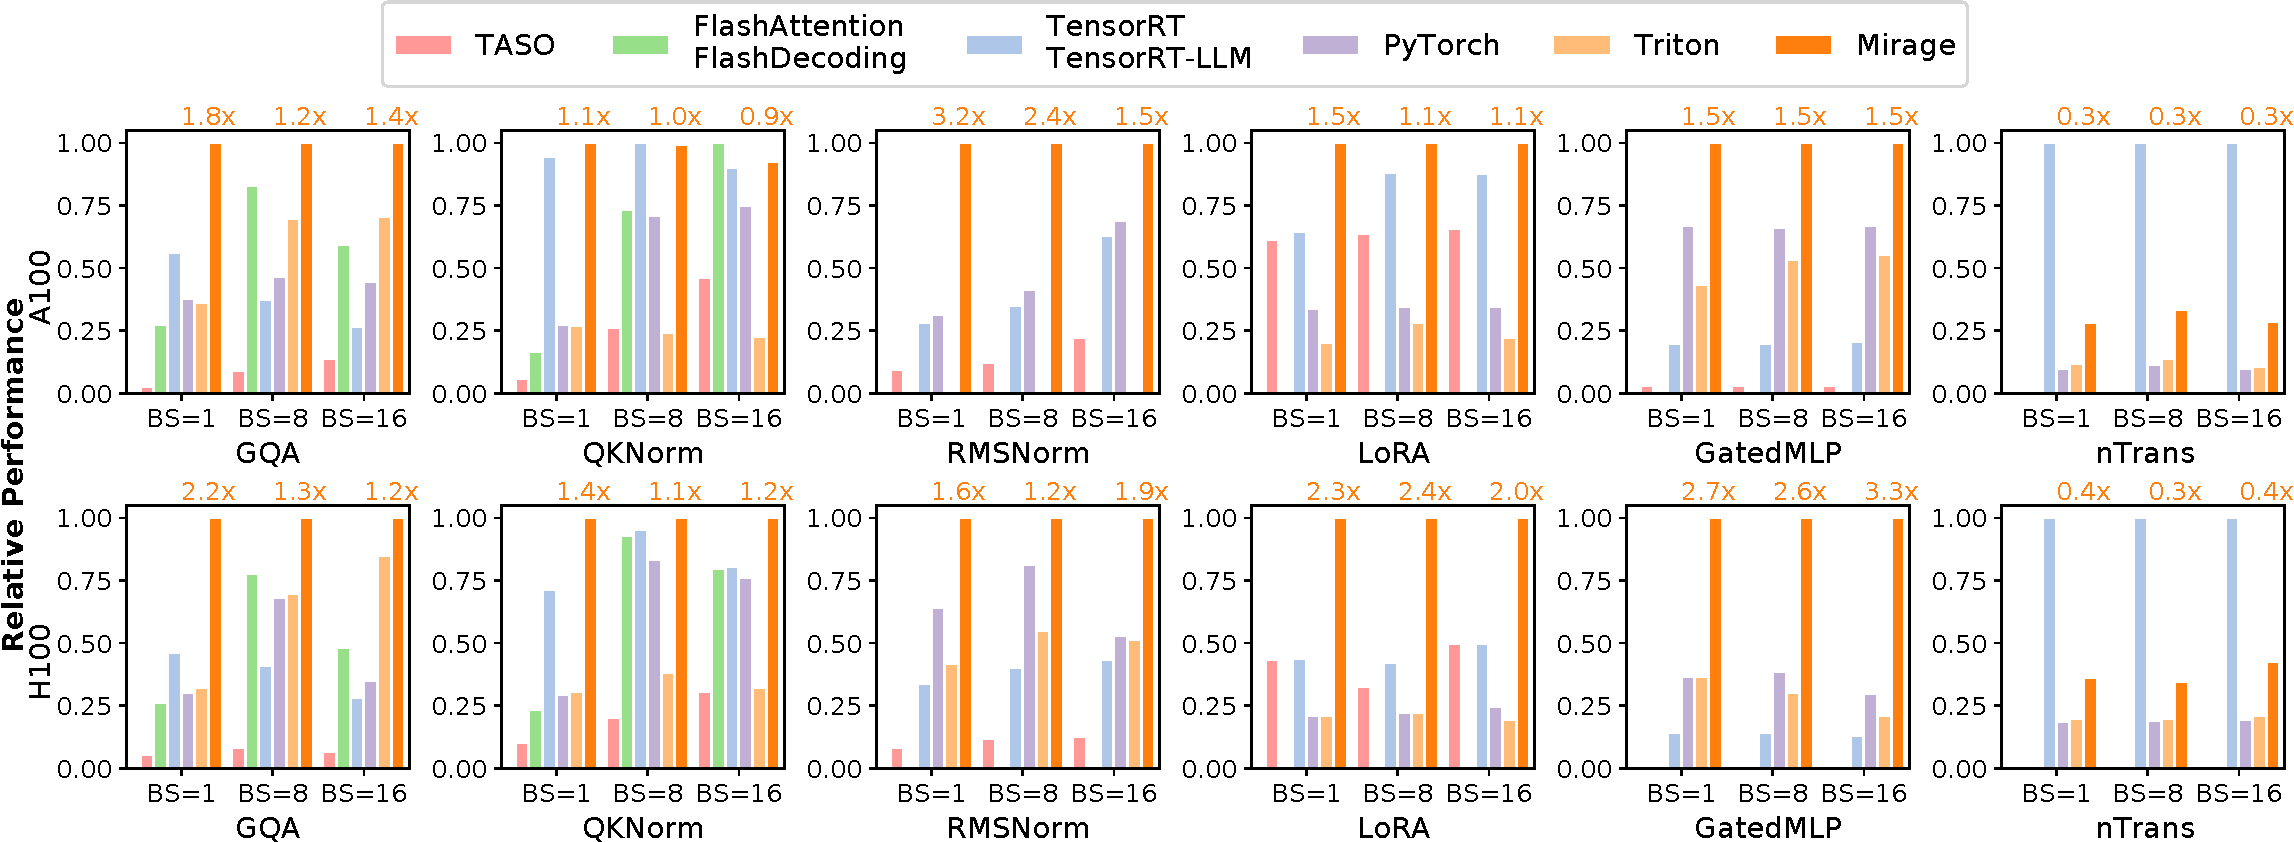
\includegraphics[width=\textwidth]{figs/benchmark-crop.pdf}
    \vspace{-1em}
    \caption{在 A100 和 H100 GPU 上对 6 个基准测试进行 \sys 与现有系统的比较。所有系统的性能均以 \sys 为基准归一化（越高越好）。\sys 柱状图上方的数字显示相对最佳基线的加速比。}
    \vspace{\captionvspace}
    \label{fig:benchmarks}
\end{figure*}

由于 \sys 是针对 \lax 程序的超级优化器，我们的评估重点关注现有 DNN 中常用的各种 DNN 基准测试，每个基准测试都是一个 \lax 程序。
这些基准测试提供了最细粒度的方式来比较 \sys 和现有系统的性能。
\Cref{tab:benchmarks} 展示了我们评估中使用的六个基准测试。
GQA、RMSNorm 和 GatedMLP 是大型语言模型（LLM）的主要构建模块。
QKNorm 在注意力之前引入查询-键归一化，以增强模型收敛性~\cite{chameleonteam2024chameleon}。
LoRA 支持对 DNN 进行低秩适配以在不同任务上进行微调。
对于 GQA，我们使用 8K 的上下文长度；对于 QKNorm，使用 4K 的上下文长度，分别对应 \llama-3-70B~\cite{grattafiori2024llama3herdmodels} 和 Chameleon-7B~\cite{chameleonteam2024chameleon} 所支持的最大上下文长度。
此外，我们还评估了 \sys 生成的核对完整 DNN 端到端性能的提升，包括 Chameleon~\cite{chameleonteam2024chameleon}、nGPT~\cite{loshchilov2024ngpt}、\llama-3~\cite{grattafiori2024llama3herdmodels} 和 LoRA~\cite{hu2021lora}。

实验在 NVIDIA A100 和 H100 GPU 上进行，每个 GPU 配有 40GB 内存。
我们的所有基准测试都能在单个 GPU 上运行，但 GQA（用于 \llama-2-70B）通常需要使用张量模型并行~\cite{Megatron} 跨四个 GPU 并行化。
因此，我们在此并行化策略下评估 GQA，其中八个键值头均等分配到四个 GPU 上。
由于 \sys 和所有基线的性能只取决于输入张量的形状，我们使用随机输入重复每个实验 1,000 次并报告平均运行时间。

我们的基准测试之一 LoRA 需要拼接操作来表达一种常见优化：通过拼接融合两个矩阵乘法。为了在 \sys 中支持这种优化，我们引入了一个新的线性运算符，接受四个输入并计算 $f(W, X, Y, Z) = (W \| X) \times (Y \| Z)$，其中 $\|$ 表示张量拼接。
该运算符等价于计算 $W \times Y + X \times Z$。
我们为该运算符定义抽象表达式如下：
$\expr(f(W, X, Y, Z)) = \eadd(\ered(k_1, \emul(\expr(W), \expr(Y))), \ered(k_2, \emul(\expr(X), \expr(Z))))$，其中 $k_1$ 和 $k_2$ 分别是 $W$ 和 $X$ 的最后一维。

除非另有说明，\sys 在核图中最多考虑 5 个运算符，在每个块图中最多考虑 11 个运算符。

\subsection{基准测试结果}
\label{subsec:benchmark_results}
\Cref{fig:benchmarks} 比较了 \sys 与现有系统在 NVIDIA A100 和 H100 GPU 上六个 DNN 基准测试上的性能。
所有系统均使用半精度浮点数运行这些 DNN 基准测试。
TASO~\cite{TASO} 和 PET~\cite{wang2021pet} 是自动生成核层次代数变换的 DNN 超级优化器。
我们报告 TASO/PET 组合基线，因为最新的 TASO 实现将 PET 的部分等价变换包含为特殊替换规则。
PyTorch~\cite{pytorch} 使用高度优化的 cuDNN 和 cuBLAS 库~\cite{cublas,cudnn} 在 GPU 上执行 DNN 运算符。
对于 PyTorch 基线，我们启用 {\tt torch.compile} 并使用 FlashAttention 核以最大化性能。
TensorRT 及其 LLM 变体 TensorRT-LLM 包含一组为常见张量运算符（如注意力~\cite{tensorrt}）手动设计和高度优化的核。
FlashAttention 及其推理变体 FlashDecoding 是用于高效注意力的手写核~\cite{dao2023flash, hong2024flashdecoding}。
最后，Triton 是一种基于调度的优化器，用于生成高性能核，已被生产系统采用，性能超过其他基于调度的方法~\cite{tillet2019triton}。
所有基线均使用 CUDA Graphs 以最小化核启动开销。

与最佳现有方法相比，\sys 通过结合代数变换、调度变换和生成新的自定义核，将这些基准测试的性能提升了最高达 $3.3\times$。\S\ref{sec:case2} 展示了 \sys 为 RMSNorm 发现的最优 \graphs。以下我们对其余基准测试进行案例研究。

\begin{figure}
    \centering
    \subfloat[现有系统中 QKNorm 和注意力的核图。]{
    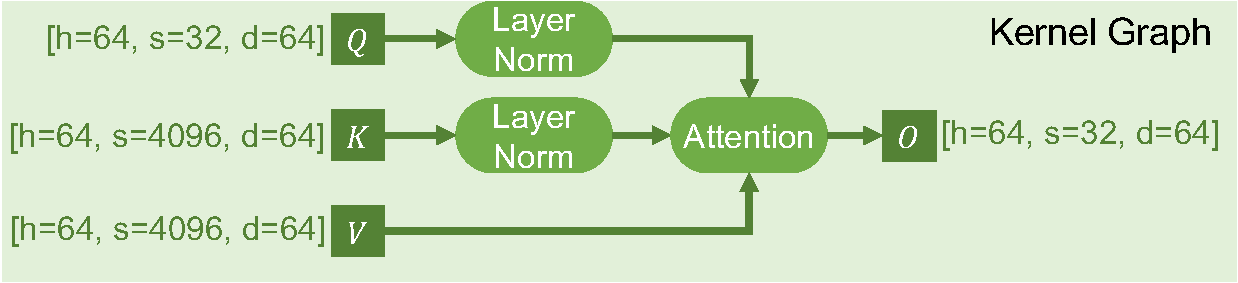
\includegraphics[scale=0.37]{figs/qknorm_attn_baseline-crop.pdf}
    \label{fig:qknorm_baseline}
    }
    \\
    \subfloat[\sys 为 QKNorm 和注意力发现的最优 \graph。]{
    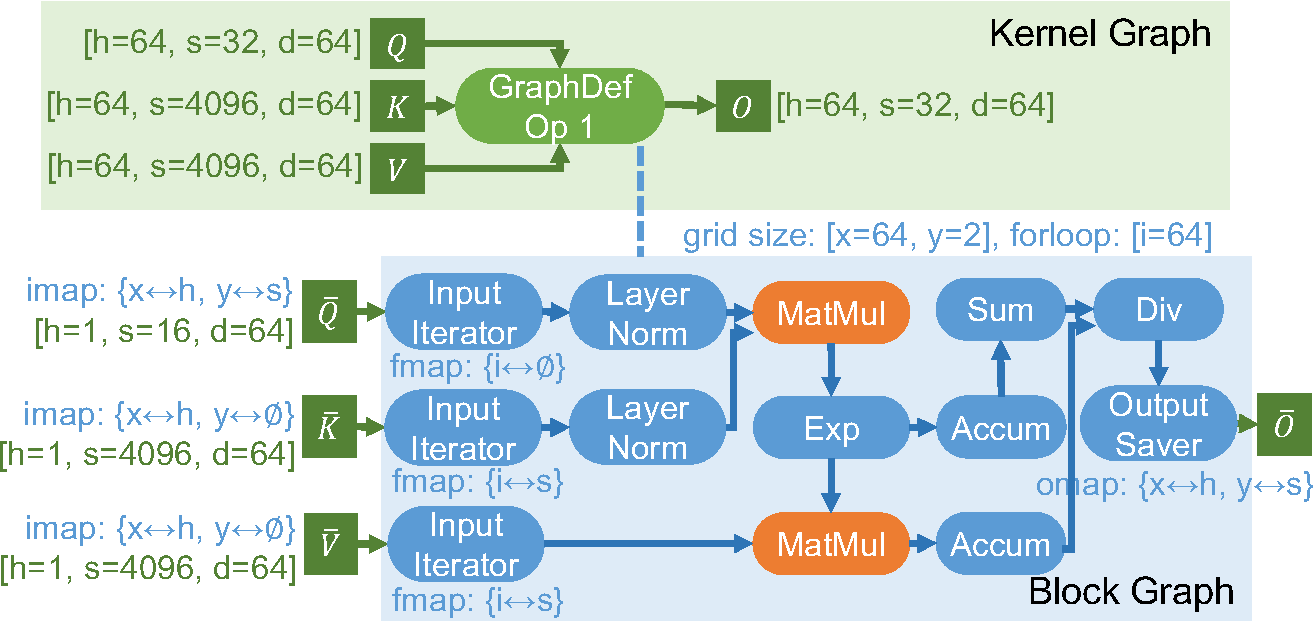
\includegraphics[scale=0.37]{figs/qknorm_attn_ours-crop.pdf}
    \label{fig:qknorm_ours}
    }
    \vspace{\captionvspace}
    \caption{比较现有优化器和 \sys 针对 QKNorm 和注意力使用的 \graphs。}
    \vspace{\captionvspace}
    \label{fig:qknorm_example}
\end{figure}

\paragraph{GQA。}分组查询注意力是 LLM 的核心组件，已被现有框架深度优化。例如，FlashAttention 和 FlashDecoding 是专家设计的注意力核，已被现有 LLM 推理系统采用~\cite{dao2023flash}。
\sys 发现了这些专家设计的核以及其他在某些场景下超越它们最高达 $2.2\times$ 的 \graphs。
加速通过以下两项在现有手写核基础上的额外优化实现。第一，当前方法依赖固定启发式策略来确定 GQA 的网格维度，在某些场景下并不最优。例如，TensorRT-LLM 在批大小为 1 和 8 时，分别以网格维度 (8, 2, 1) 和 (8, 2, 8) 启动 GQA 核。然而，这两种配置都无法充分利用 A100（108 个 SM）和 H100（132 个 SM）GPU 上的所有 SM。
相比之下，\sys 自动为每个 \graph 搜索最佳网格维度，从而实现全部 SM 利用率。
进一步的消融实验表明，当使用与 TensorRT-LLM 相同的网格维度时，\sys 发现的最优 \graph 的性能降低了 18\%。

第二，现有方法使用固定的张量维度来跨线程块并行化 GQA。例如，FlashAttention~\cite{dao2023flash} 沿{\em 样本}、{\em 头}和{\em 查询序列}维度并行化注意力，而 FlashDecoding 和 TensorRT-LLM 则利用{\em 样本}、{\em 头}和{\em 键值序列}维度。这两种策略对于具有多头的传统多头注意力很高效，但对于头数较少的 GQA 则不够最优。
相比之下，\sys 通过在样本、KV 头、查询序列和键值序列维度之间进行选择，自动选择最高效的并行化策略。此外，\sys 为不同的注意力场景生成不同的 \graphs，与现有系统使用的启发式策略相比，最多可减少 $7\times$ 的设备内存访问。

在现有系统中实现 \sys 的 \graphs 是可行的，但需要大量工程工作来支持针对不同场景的不同核。相比之下，\sys 会自动生成它们并验证其正确性。

\paragraph{QKNorm。}为减少模型发散，近期一些 DNN 在 Transformer 架构中引入了查询-键归一化（QKNorm）~\cite{chameleonteam2024chameleon}。QKNorm 在注意力之前对查询和键向量应用层归一化，如 \Cref{fig:qknorm_baseline} 所示。这些额外的归一化层尚未被现有注意力实现（如 FlashAttention 和 TensorRT-LLM）支持，需要为归一化和注意力分别启动独立的核。

\Sys 自动发现了一个将 QKNorm 和注意力计算集成到自定义核中的 \graph，如 \Cref{fig:qknorm_ours} 所示。该 \graph 重新组织了注意力计算以支持与两个层归一化的融合，避免将中间结果写入 GPU 设备内存，将核执行时间减少了最高达 $1.4\times$。

\begin{figure}
    \centering
    \subfloat[现有系统中 LoRA 的核图。]{
    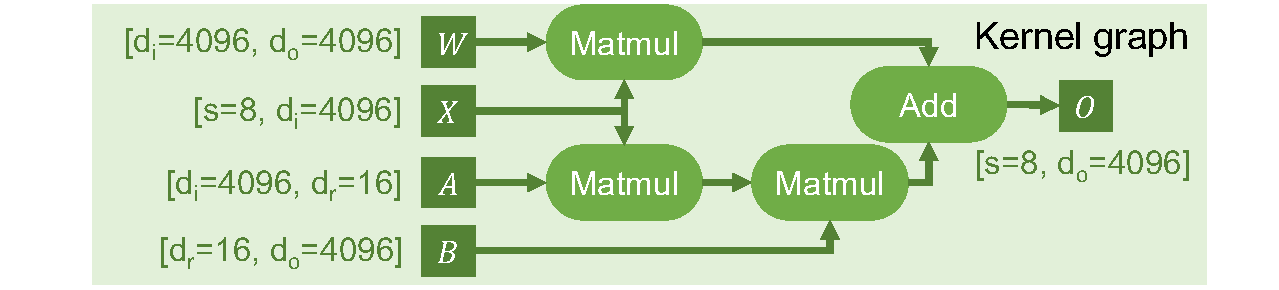
\includegraphics[scale=0.38]{figs/lora_baseline.pdf}
    \label{fig:lora_baseline}
    }
    \\
    \subfloat[\sys 为 LoRA 发现的最优 \graph。]{
    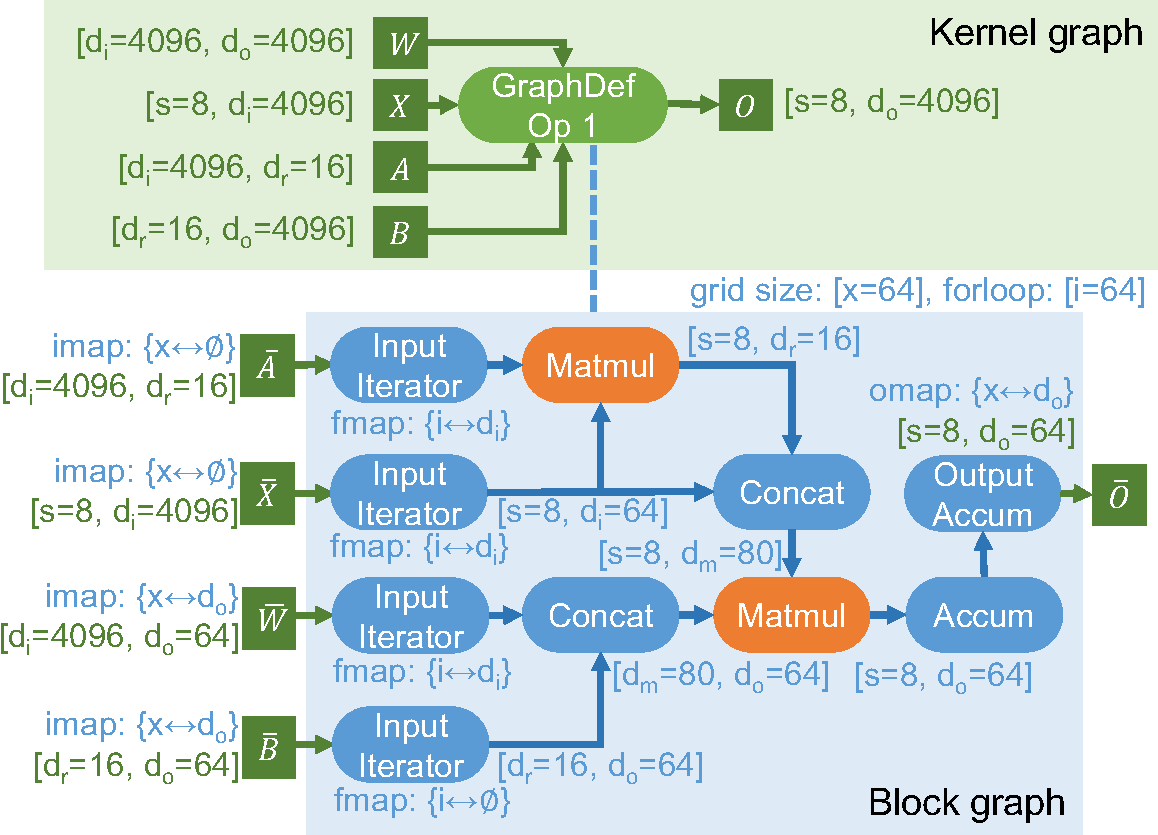
\includegraphics[scale=0.38]{figs/lora_ours_v2-crop.pdf}
    \label{fig:lora_ours}
    }
    \vspace{\captionvspace}
    \caption{比较现有优化器和 \sys 针对 LoRA 使用的张量程序：$O = W \times X + B \times A \times X$。注意矩阵 $A$ 和 $B$ 均为低秩矩阵。}
    \vspace{\captionvspace}
    \label{fig:lora_example}
\end{figure}

\paragraph{LoRA。}
低秩适配（LoRA）向预训练 DNN 的线性运算符引入一对低秩适配器，以提升其在下游任务上的性能。
现有张量程序优化器为原始线性运算符和 LoRA 引入的两个额外线性运算符分别启动独立的核（\Cref{fig:lora_baseline}），由于这些 LoRA 运算符涉及极少量计算，这会引入较高的核启动开销。
\Cref{fig:lora_ours} 展示了 \sys 为 LoRA 发现的最优 \graph，它将三个 {\tt Matmul} 和随后的 {\tt Add} 融合到单个核中。\sys 利用以下代数变换将计算重新组织为两个块级 {\tt Matmul}：$W \times X + B \times A \times X = (W \| B) \times \big(X \| (A\times X)\big)$。\Cref{fig:lora_ours} 中的 {\tt Concat} 不涉及任何计算，通过更新 GPU 共享内存中的张量偏移量来实现。
该 \graph 将 LoRA 的执行代价降低了 $1.1$--$2.4\times$。

\begin{figure}
    \centering
    \subfloat[GatedMLP 的核图。]{
    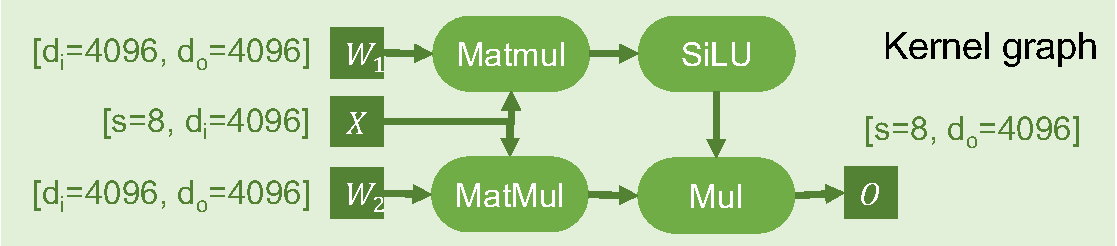
\includegraphics[scale=0.4]{figs/gated_mlp_baseline-crop.pdf}
    \label{fig:mlp_baseline}
    }
    \\
    \subfloat[\sys 为 GatedMLP 发现的最优 \graph。]{
    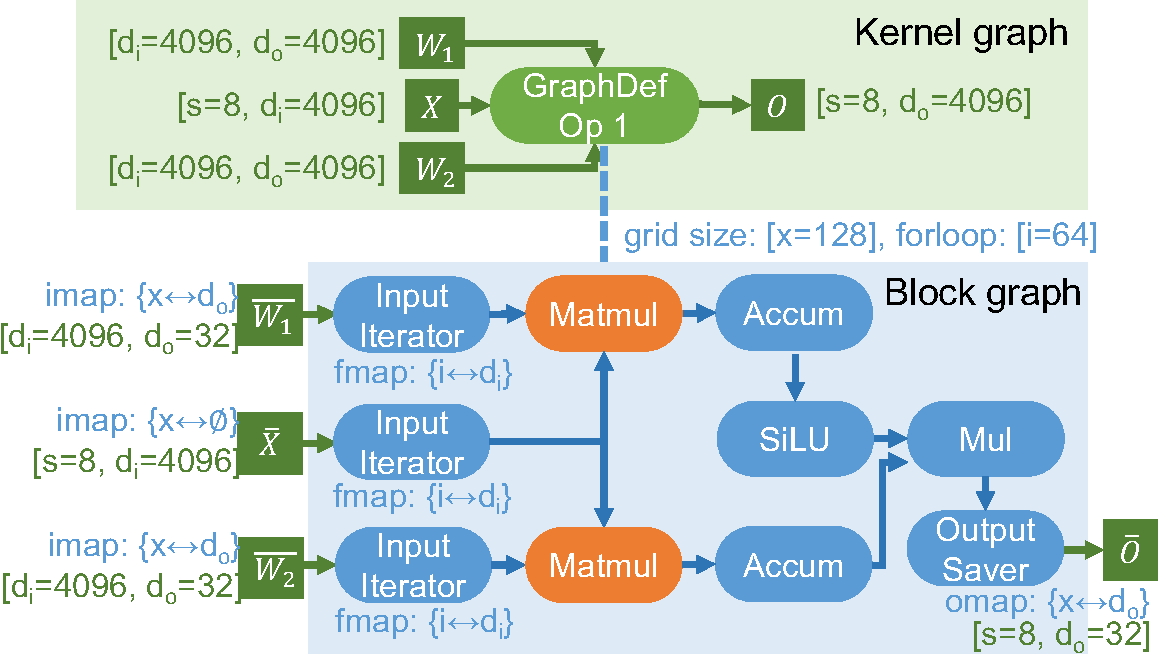
\includegraphics[scale=0.4]{figs/gated_mlp_ours-crop.pdf}
    \label{fig:mlp_ours}
    }
    \vspace{\captionvspace}
    \caption{比较现有优化器和 \sys 针对 GatedMLP 使用的 \graphs。}
    \vspace{\captionvspace}
    \label{fig:mlp_example}
\end{figure}

\paragraph{GatedMLP。}
门控多层感知器广泛用于 DNN 中以捕获非线性表示。
我们使用 Falcon-7B~\cite{falcon40b} 中引入的 GatedMLP 配置，其核图如 \Cref{fig:mlp_baseline} 所示。
现有张量程序优化器通常将两个 {\tt Matmul} 融合在单个核中以减少 GPU 设备内存访问，因为输入张量 $X$ 只需加载一次。
然而，这种方法仍需启动多个核并将中间结果——具体来说是两个 {\tt Matmul} 的输出——存储在设备内存中，因为 {\tt SiLU} 激活函数和逐元素乘法没有与 {\tt Matmul} 融合。

相比之下，\sys 发现的最优 \graph（\Cref{fig:mlp_ours}）在同一块图中并行执行两个 {\tt Matmul}，并将其余计算（即 {\tt SiLU} 和 {\tt Mul}）作为同一块图内的后处理步骤进行融合。这种方法在 A100 GPU 上实现了 $1.5\times$ 的加速，在 H100 GPU 上实现了 $2.7$--$3.3\times$ 的加速。

\paragraph{nTrans。}
为了加速模型训练，nGPT 引入了归一化 Transformer，它对 Transformer 中的所有中间结果进行归一化~\cite{loshchilov2024ngpt}。形式上，计算定义为 $y = \texttt{Norm}(x + \alpha (\texttt{Norm}(h - x)))$，其中 {\tt Norm} 是归一化层，$x$、$h$ 和 $\alpha$ 是输入张量。由于 nTrans 将归一化、逐元素加法和乘法交错进行，现有系统为 nTrans 启动三个独立的核。\Sys 自动发现了一个将计算融合到单个核中并将所有中间结果存储在 GPU 共享内存中的 \graph。\Sys 优于其他基线，但比 TensorRT 慢。这一性能差距是因为 \Sys 在图定义核中为每个张量从全局内存加载数据到共享内存再写回。这种设计提高了内存效率并支持异步流水线，但对于计算量轻的核，这些内存传输的开销可能主导核的运行时间。
为了缓解这一开销，我们计划扩展 \sys 以支持在数据加载时绕过共享内存，从而避免不必要的数据移动。

\begin{figure}
    \centering
    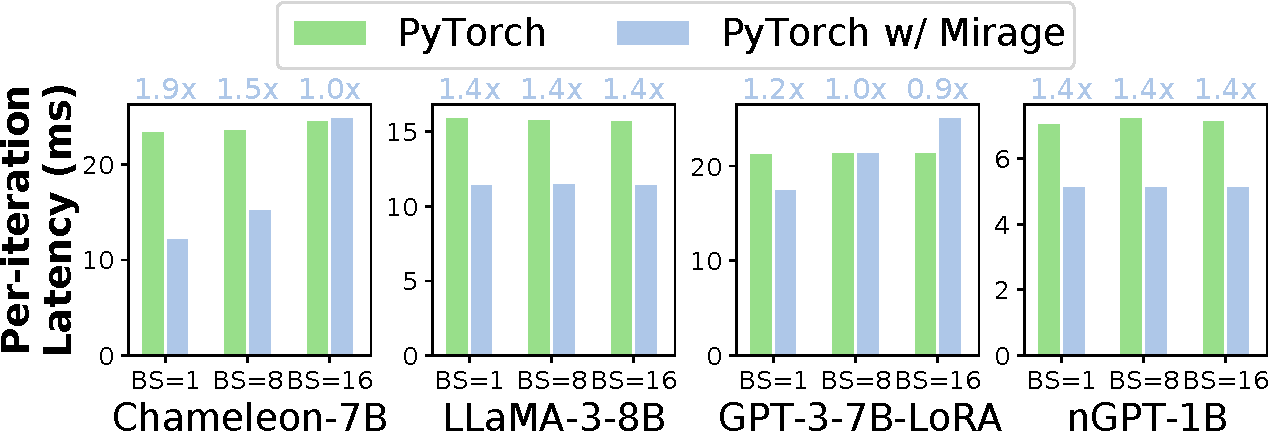
\includegraphics[width=\columnwidth]{figs/end2end-crop.pdf}
    \caption{比较 PyTorch 和使用 \sys 生成核的 PyTorch 的端到端推理性能。}
    \label{fig:end_to_end_models}
\end{figure}

\subsection{端到端结果}
除了微基准性能，我们还评估了 \sys 生成的核对常用 DNN 端到端延迟的影响。\sys 支持即时编译和部署，其生成的核可以直接集成到 PyTorch 程序中。我们在四个 DNN 模型上比较了使用原生手写 CUDA 核的 PyTorch 和使用 \sys 生成核的 PyTorch。\Cref{fig:end_to_end_models} 展示了结果。\sys 通过自动生成高度优化的核，将这些模型的端到端延迟减少了 $0.9$--$1.9\times$。这一改进只需对 PyTorch 程序进行几行代码修改即可实现。

\subsection{搜索时间}

\begin{table}
    \centering
    \caption{\sys 加速 \graph 生成技术的消融实验。我们评估多线程和抽象表达式对 RMSNorm 搜索时间的影响。}
    \vspace{\captionvspace}
    \footnotesize
    \label{tab:search_time}
    \begin{tabular}{c|r|r|r}
    \toprule
    {\bf 块图中算子} & {\bf \sys} & {\bf \sys（无} & {\bf \sys（无}\\
    {\bf 最大数量} & {\bf } & {\bf 多线程）} & {\bf 抽象表达式）} \\
    \midrule
    $5$ & $11$ 秒 & $58$ 秒 & $768$ 秒 \\
    $6$ & $16$ 秒 & $93$ 秒 & $19934$ 秒 \\
    $7$ & $22$ 秒 & $150$ 秒 & $> 10$ 小时 \\
    $8$ & $24$ 秒 & $152$ 秒 & $> 10$ 小时 \\
    $9$ & $26$ 秒 & $166$ 秒 & $> 10$ 小时 \\
    $10$ & $26$ 秒 & $166$ 秒 & $> 10$ 小时 \\
    $11$ & $28$ 秒 & $183$ 秒 & $> 10$ 小时 \\
    \bottomrule
    \end{tabular}
    \vspace{\captionvspace}
\end{table}

在我们的评估中，\sys 优化一个 \lax 程序最多需要 4 小时。这一优化是在目标硬件上部署之前的一次性代价。
本小节提供 \sys 搜索过程的详细结果和消融实验，重点分析其技术如何在保持低搜索时间的同时支持对大型 \graphs 的探索。
具体地，我们评估了两项技术的影响：通过抽象表达式剪枝（\S\ref{subsec:abstract_expression}）和多线程。
\Cref{tab:search_time} 报告了 RMSNorm 在不同块图最大运算符数量下的搜索时间。

多线程显著缩短了搜索时间，而通过抽象表达式剪枝对 \sys 的可扩展性至关重要。
具体地，剪枝技术使 \sys 能够探索每个块图最多包含 11 个运算符的 \graphs，而禁用抽象表达式剪枝则将 \sys 限制在 10 小时搜索窗口内只能处理最多 6 个运算符的块图。
需要注意的是，发现 \Cref{fig:mugraph} 所示的 RMSNorm 优化 \graph 需要探索包含 11 个运算符的块图。

\subsection{优化手段消融实验}

\begin{figure}
    \centering
    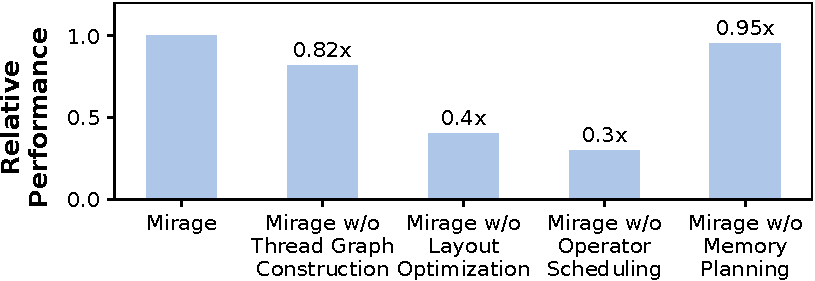
\includegraphics[width=\columnwidth]{figs/ablation-crop.pdf}
    \vspace{\captionvspace}
    \caption{Mirage 中优化手段的消融实验。我们在批大小为 1 的 GQA 基准测试上，在 A100 GPU 上评估分别禁用每项优化时的性能下降。}
    \vspace{\captionvspace}
    \label{fig:ablation-optimization}
\end{figure}

我们进行消融实验，评估线程图构建和 \S\ref{sec:optimizer} 中介绍的优化手段（包括布局优化、运算符调度和内存规划）的影响。具体地，我们测量在独立禁用每项优化时 \sys 发现的最优 \graph 的性能下降情况。实验在批大小为 1 的 GQA 基准测试上的 A100 上进行。结果如 \Cref{fig:ablation-optimization} 所示，禁用任何单项优化都会导致 $5\%$ 到 $70\%$ 不等的性能下降。
